%------------------------------------------------------------
% Description : Куски теормеха --- получше 
% Author      : Iliya Tikhonenko <iliya.t@mail.ru>
% Created at  : Fri Jun 16 18:12:20 MSK 2017
%------------------------------------------------------------
\documentclass[timbord]{longnotes}
\usepackage{tmath}
\usepackage{cussymb}
\graphicspath{{img/}}

\makeatletter
\makeatother

\begin{document}
\chapter{Кинематика точки}

\setcounter{paragraph}{1}
\paragraph{Косоугольные координаты}

Здесь можно немного добавить строгости, а то ничерта не понятно.
Пусть $V$~--- евклидово пространство (линейное со скалярным произведением).
Как нам определяли, $g_{ik} = \v{e_i} \cdot \v{e_k}$,
\[
   \v a \cdot \v b  = \sum_{ij}  a^i b^j g_{ij}
\]
Здесь $a^k$~--- коэффициенты разложения по $\v{e_k}$~--- называются контравариантными координатами.

Пусть $V^*$~--- сопряжённое к $V$, его базисом являются координатные функции
$\v*{f_k} \that \v*{f_k}(\v x) = x^k$. 
Поскольку задано скалярное произведение, задан канонический изоморфизм $V \to V^*$.
Нам, правда, потребуется $V^* \to V$.

Введём ещё одну систему \emph{векторов} в $V$ : $\v{e^k} = \v*{f_k^*}$, то есть 
$\v*{f_k}(\v x) = \v{e^k} \cdot \v x$. 
Она и называется взаимным
базисом, коэффициенты разложения по ней~--- ковариантные координаты.
Из линейности скалярного произведения, ровно такие же координаты будут у соответствующей
формы в $V^*$.
Линейную независимость легко получить из ЛНЗ $\v*{f_k}$, a
раз их $\dim V$, то полученные векторы являются базисом.

Так что можно сформулировать правило:
\begin{itemize}
  \item Контравариантные координаты~--- коэффициенты разложения по базису линейного пространства.
  \item Ковариантные координаты~--- коэффициенты разложения по базису пространства линейных форм.
\end{itemize}
Ещё можно определить $g^{ij} = \v{e^i \cdot e^j}$, и перенести это на 
соответствующие линейные формы. Обобщая дальше, можно вообще сказать, что $g_i^k = \delta_{ij}$.
Тогда $g$ будет задавать действие формы на вектор. Вроде физикам это зачем-то надо.

А после тирады выше уже развлекаться с индексами.

\begin{prop}
  $\v{e^k} \cdot \v{e_j} = \delta_{kj}$
\end{prop}
\begin{lproof}
  Следует из определения координатной функции, ведь $\v{e^k} \cdot \v x = \v*{f_k}(\v x)$
\end{lproof}

\begin{prop}
  $\v a\cdot \v b = \sum_i a^i b_i$
\end{prop}

\begin{prop}
  Пусть $\v r = \sum_k \xi^k \v {e_k}$ и $=\sum_k\xi_k \v{e^k}$.
  Тогда $\xi_k = \v r \cdot \v{e_k} = \sum_j \xi^j g_{jk}$
\end{prop}
\begin{lproof}
  Ну, $\v{r} \cdot \v{e_k} = \dsum_j \xi_j \, \v{e^j}\cdot \v{e_k} 
  = \sum_j \xi_j \,\delta_{jk} = \xi_k$. Вроде всё.
\end{lproof}

Аналогичная ситуация с $\xi^k$.
\begin{prop}
  $\xi^k = \v{r\cdot e^k} = \sum_j \xi_j g^{jk}$.
\end{prop}

\begin{prop}
\[
  \v{e^k} = \sum_j g^{jk} \v{e_j}, \quad \v{e_k} = \sum_j g_{jk} \v{e^j}
\]
\begin{lproof}
  Первое домножить на $\v{e^i}$, второе на $\v{e_i}$.
\end{lproof}
\end{prop}
\begin{prop}
  $\sum_{i} g^{i\ell}g_{ik} = \delta_{\ell k}$
\end{prop}
\begin{lproof}
%   Дельта-символ, как и дельта-функция проявляется в сумме (или интеграле).
  \[
    \sum_{i} g^{i\ell}g_{ik} = \sum_i g^{i\ell} \v{e_i \cdot e_k} = \v{e^\ell}\cdot \v{e_k} =
    \delta_{\ell k}
  \]  
\end{lproof}


Как видно, когда определения безкоординатные, жызнъ прекрасна!. 
\note{тут не опечатка, а отсылка к известной картинке \texttt{;)}}
\setcounter{paragraph}{12}
\paragraph{Кинематический винт}

При переходе между полюсами, угловая скорость не меняется, в отличие от линейной.
Давайте это обоснуем.

\begin{minipage}{0.28\linewidth}
\vspace{1em}
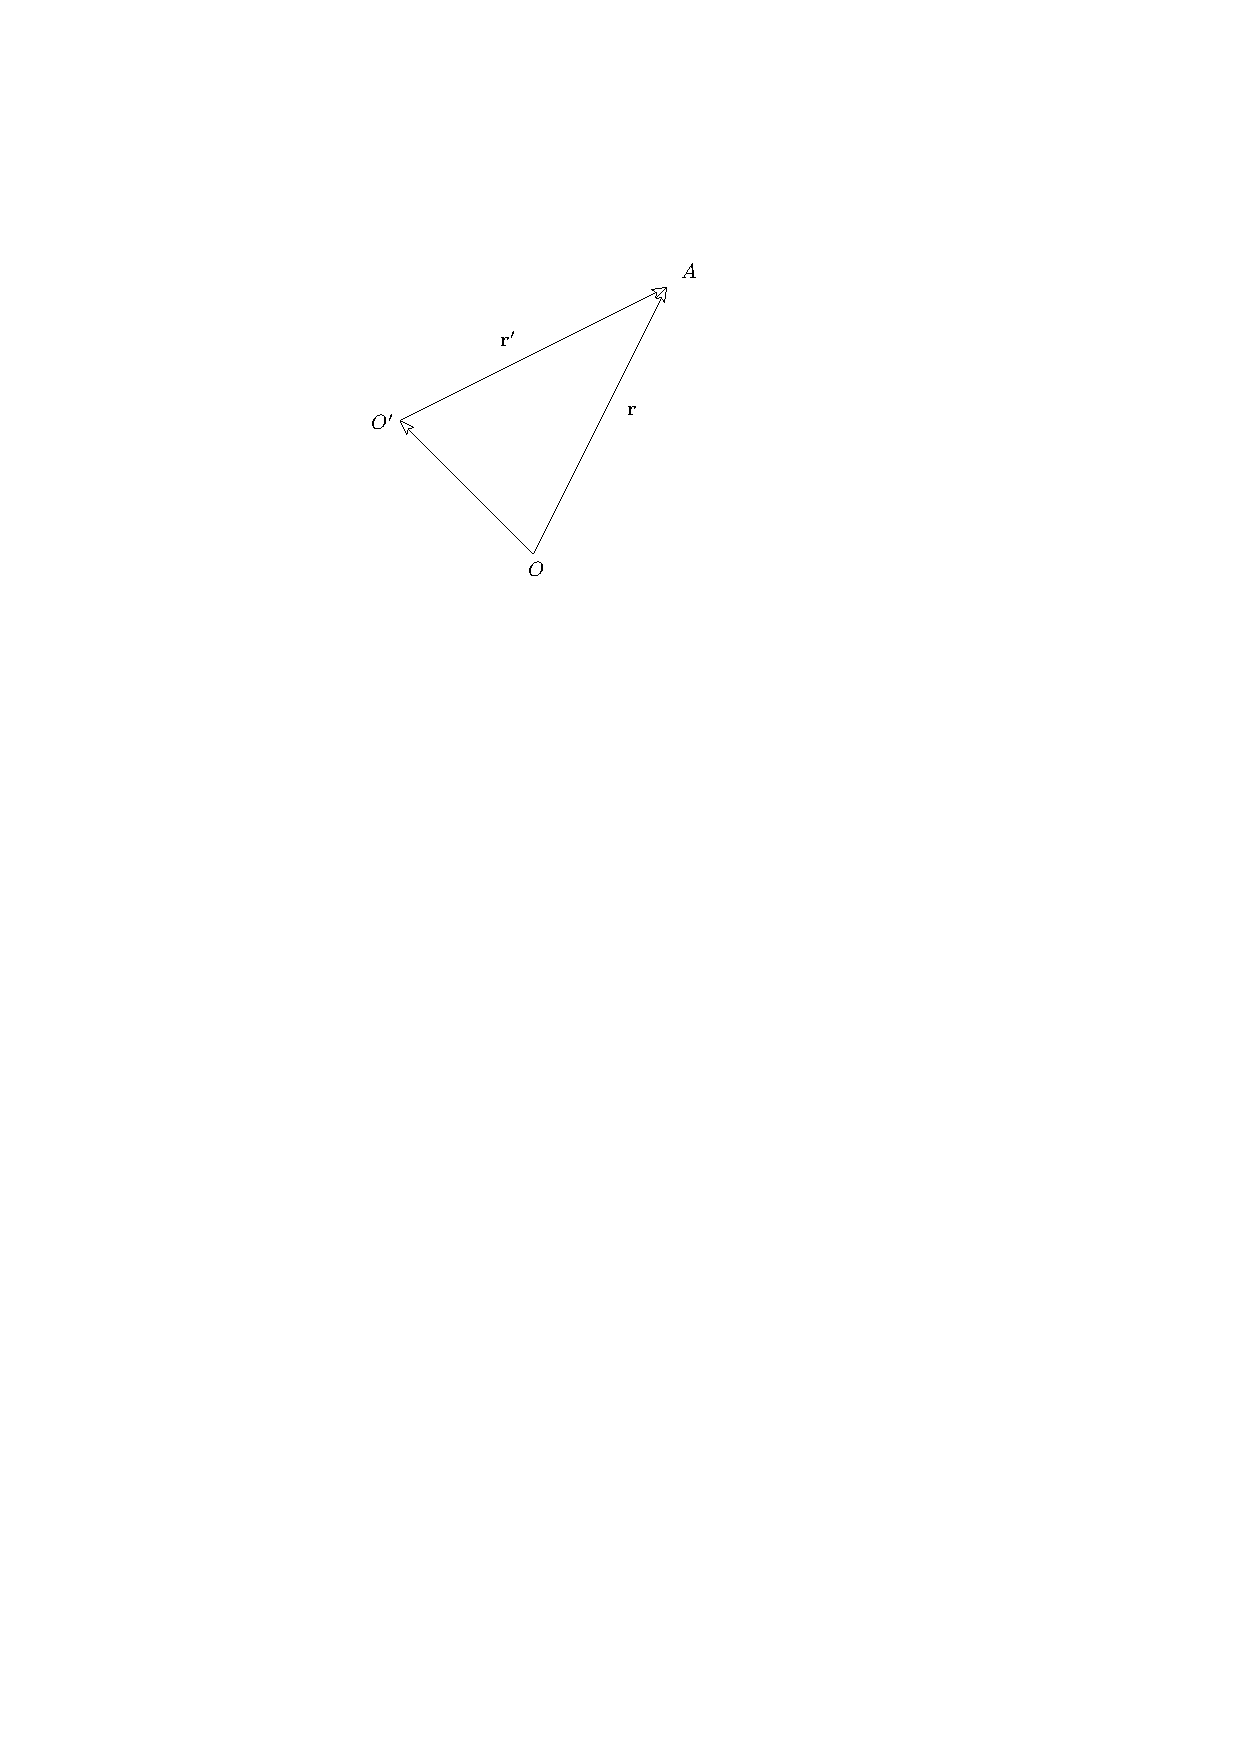
\includegraphics[scale=1]{kinscrew}
\vspace{1em}
\end{minipage} \hfill
\begin{minipage}{0.68\linewidth}
$\displaystyle
\left\{
\begin{aligned}
  \v v &= \v{v_0} + \v \omega \times \v{r} = \v{v_0'} + \v{\omega'} \times \v{r'}\\
  \v {v_0'} &= \v{v_0} + \v \omega \times \ov{->} {OO'} \\
  \v r' &= -\ov{->} {OO'} + \v r \\
\end{aligned}\right. \Rightarrow 
\begin{aligned}
  \v\omega \times (\v r - \ov{->} {OO'} ) &= \v{\omega '} \times ( - \ov{->} {OO'} + \v r) \\
                                          &\Leftrightarrow \\
  (\v \omega - \v {\omega'} ) \times ( r- \ov{->}{OO'} ) &= 0
\end{aligned}
$
\end{minipage}
Смещаться можно как угодно, так что угловые скорости равны.

Теперь про кинематический винт. При обычном винтовом движении, $\v v_0 \coori \v\omega $,
все точки на оси просто движутся со скоростью $\v v_0$, для них $\v \omega \times \v v =0$.

Теперь найдём множество таких точек, что $\v w \times \v v = 0$ в произвольном случае.
\[
  \v \omega \times \v v_0 + \v \omega \times (\v \omega \times \v r) = 0
\]
Первый член~--- не изменяется в ходе перемещений по телу при зафиксированном времени.
Если продифференцировать по $\v r$, то $\v \omega \times (\v \omega \times \v {\del r}) = 0$, 
то есть приращение $r$ всегда $\coori \v \omega $. Так что это прямая. Назовём её $\ell_k$.

Собственно, пара $(\omega, \v v)$, где $\v v\v =v(\v r), \v r \in \ell_k$ и называется кинематическим
винтом. Если перенести полюс на $\ell_k$, то движение тела сильно похоже на винтовое.

\paragraph{Плоское движение}
не сюда.

\appendix
\chapter{Обозначения}
\begin{description}
  \item[$\v*{f}$]~--- линейная форма. \hfill$\langle$\verb+\mathrm f+$\rangle$
  \item[$\v{x}$]~--- вектор. \hfill$\langle$\verb+\mathbf x+$\rangle$
\end{description}
\end{document}
% vim:tw=100 cc=100
